    \documentclass[letterpaper,11pt]{article}

    \usepackage{fullpage}
    \usepackage[usenames,dvipsnames]{color}
    \usepackage[pdftex]{hyperref}
    \usepackage{tabularx}
\usepackage{booktabs}
\usepackage{amsmath}
\usepackage{multirow}
\usepackage{layouts}
\usepackage{array}
\usepackage{pgf}
\usepackage{tikz}
\usetikzlibrary{positioning}
\usetikzlibrary{arrows,automata}
 \usepackage{graphicx}

    \hypersetup{
	colorlinks,%
	citecolor=black,%
	filecolor=black,%
	linkcolor=black,%
	urlcolor=mygreylink     % can put red here to visualize the links
    }
   
    \definecolor{mygrey}{gray}{.85}
    \definecolor{mygreylink}{gray}{.30}
    \textheight=8.6in
    \raggedbottom
    \raggedright
    \setlength{\tabcolsep}{0in}
    \addtolength{\oddsidemargin}{-0.375in}
    \addtolength{\evensidemargin}{0.375in}
    \addtolength{\textwidth}{0.5in}
    \addtolength{\topmargin}{-.375in}
    \addtolength{\textheight}{0.75in}

    \newcommand{\resitem}[1]{\item #1 \vspace{-2pt}}
    \newcommand{\resheading}[1]{{\large \colorbox{mygrey}{\begin{minipage}{\textwidth}{\textbf{#1 \vphantom{p\^{E}}}}\end{minipage}}}}
    \newcommand{\ressubheading}[4]{
    \begin{tabular*}{6.5in}{l@{\extracolsep{\fill}}r}
		    \textbf{#1} & #2 \\
		    \textit{#3} & \textit{#4} \\
    \end{tabular*}\vspace{-6pt}}
  
    \begin{document}

\begin{center}
{\LARGE \textbf{Machine Learning: Pattern Recognition}}\\ [1em]
\end{center}
\newcommand{\mywebheader}{
    \begin{tabular}{@{}p{5in}p{4in}}
		{\resheading{Report Lab 1}} & {\Large 11 September, 2012}\\\vspace{0.2cm}
	    \end{tabular}}
    \mywebheader
    
    	\begin{center}
    	{\Large By:} \\ \vspace{0.1cm}
	    {\Large Paris Mavromoustakos} \\  \vspace{0.1cm}
	    {\Large Georgios Methenitis} \\ \vspace{0.1cm}
	    {\Large Marios Tzakris}
	    \end{center}

  
  \section*{Introduction}
  The purpose of this lab assignment was to apply a k-Nearest-Neighbours classification algorithm on a given set of datapoints. To achieve this we had to become familiar with the Matlab environment, including the Netlab package. The Netlab package is a complete suit of matlab functions implementing machine learning techniques.
 
 \section*{Exercise 1}
 First of all, we loaded a given data file (twoclass.mat) which contained two classes of two-dimensional datapoints.Before creating both the training and test sets, we shuffled the two matrices in order to create groups of random datapoints. The training set consists of 75\% of class A's datapoints appended to 75\% of class B's datapoints, while the test set contains the remaining25\% of both classes. Figure \ref{fig:1} presents the plot results of the training set. Datapoints of different classes are depicted with different symbols and colors. Figure \ref{fig:2} presents the plot results of the test set.
 
 \begin{figure}[h!]
\centering
  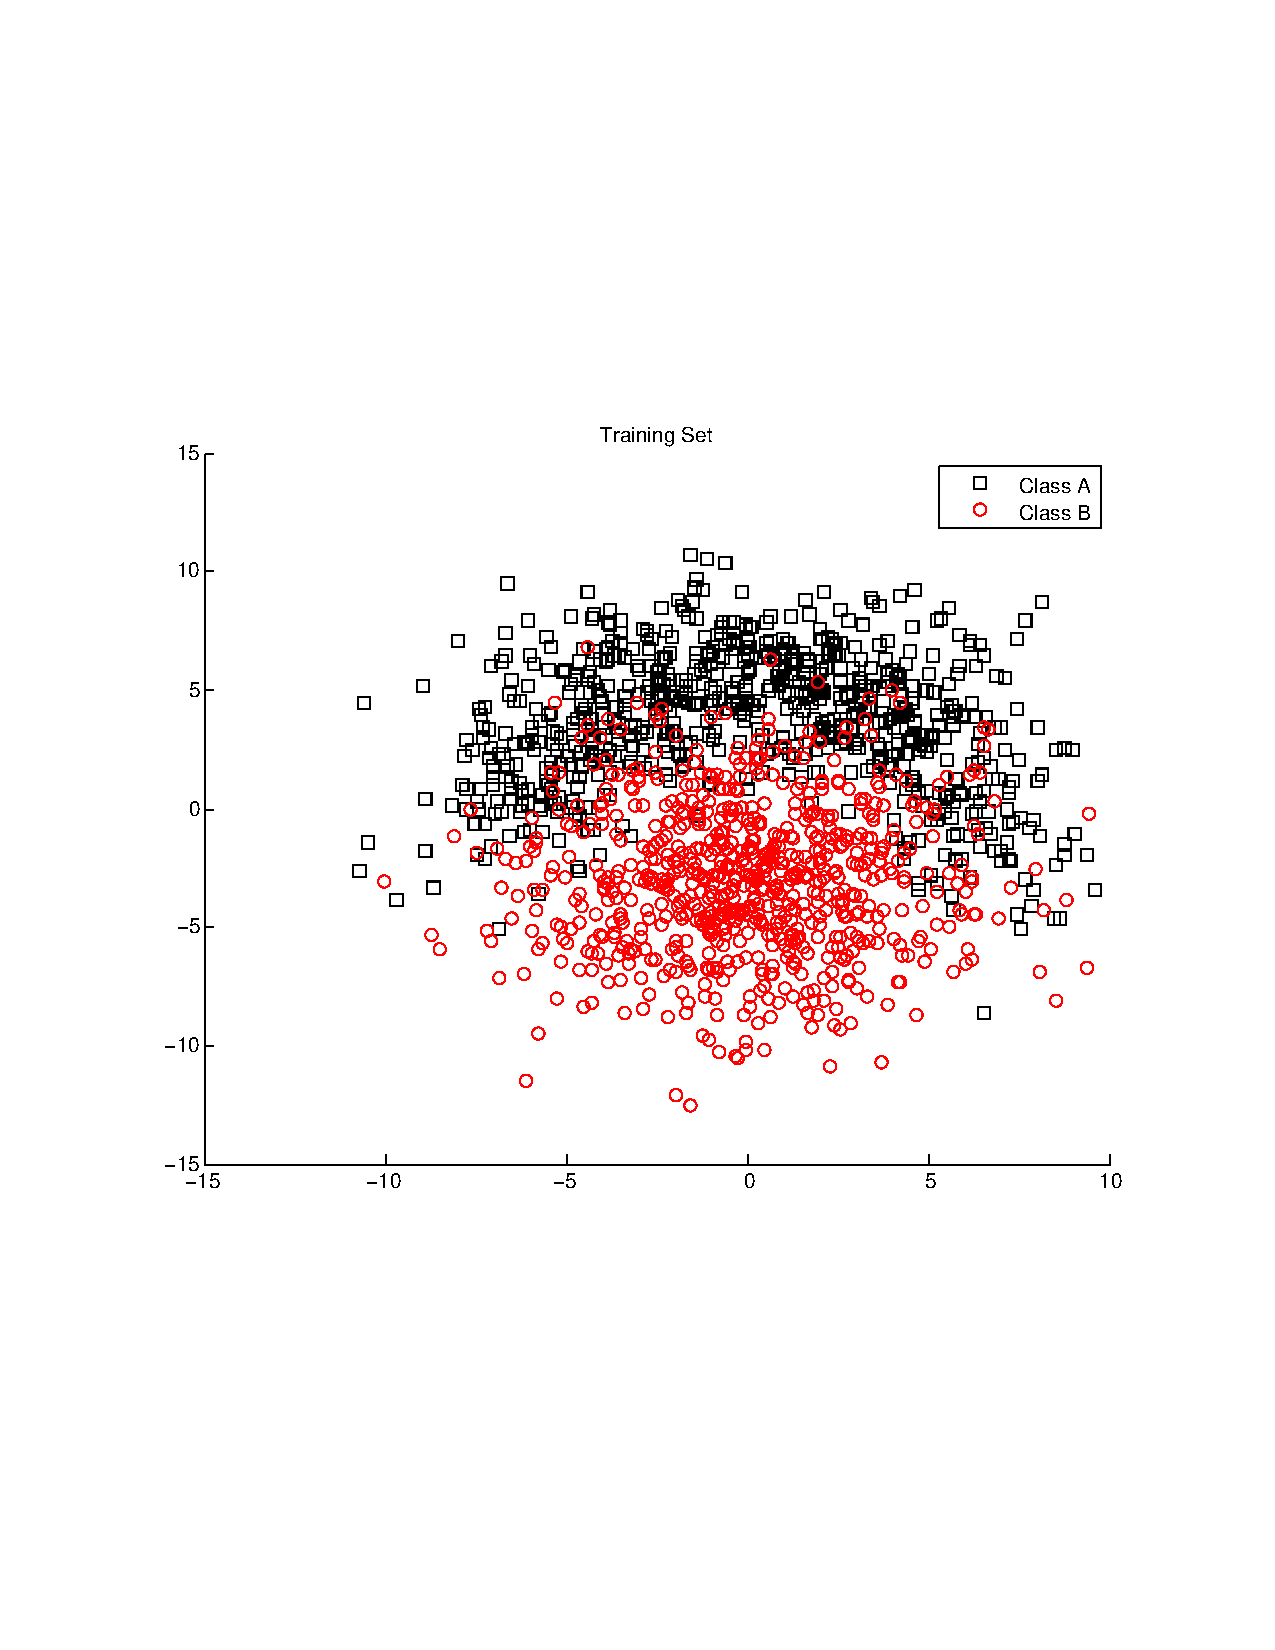
\includegraphics[trim = 0cm 7cm 0cm 7cm, clip, width=0.8\textwidth]{figures/TrainingSet.pdf}
  \caption{Training Set.}
  \label{fig:1}
\end{figure}
 
  \begin{figure}[t!]
\centering
  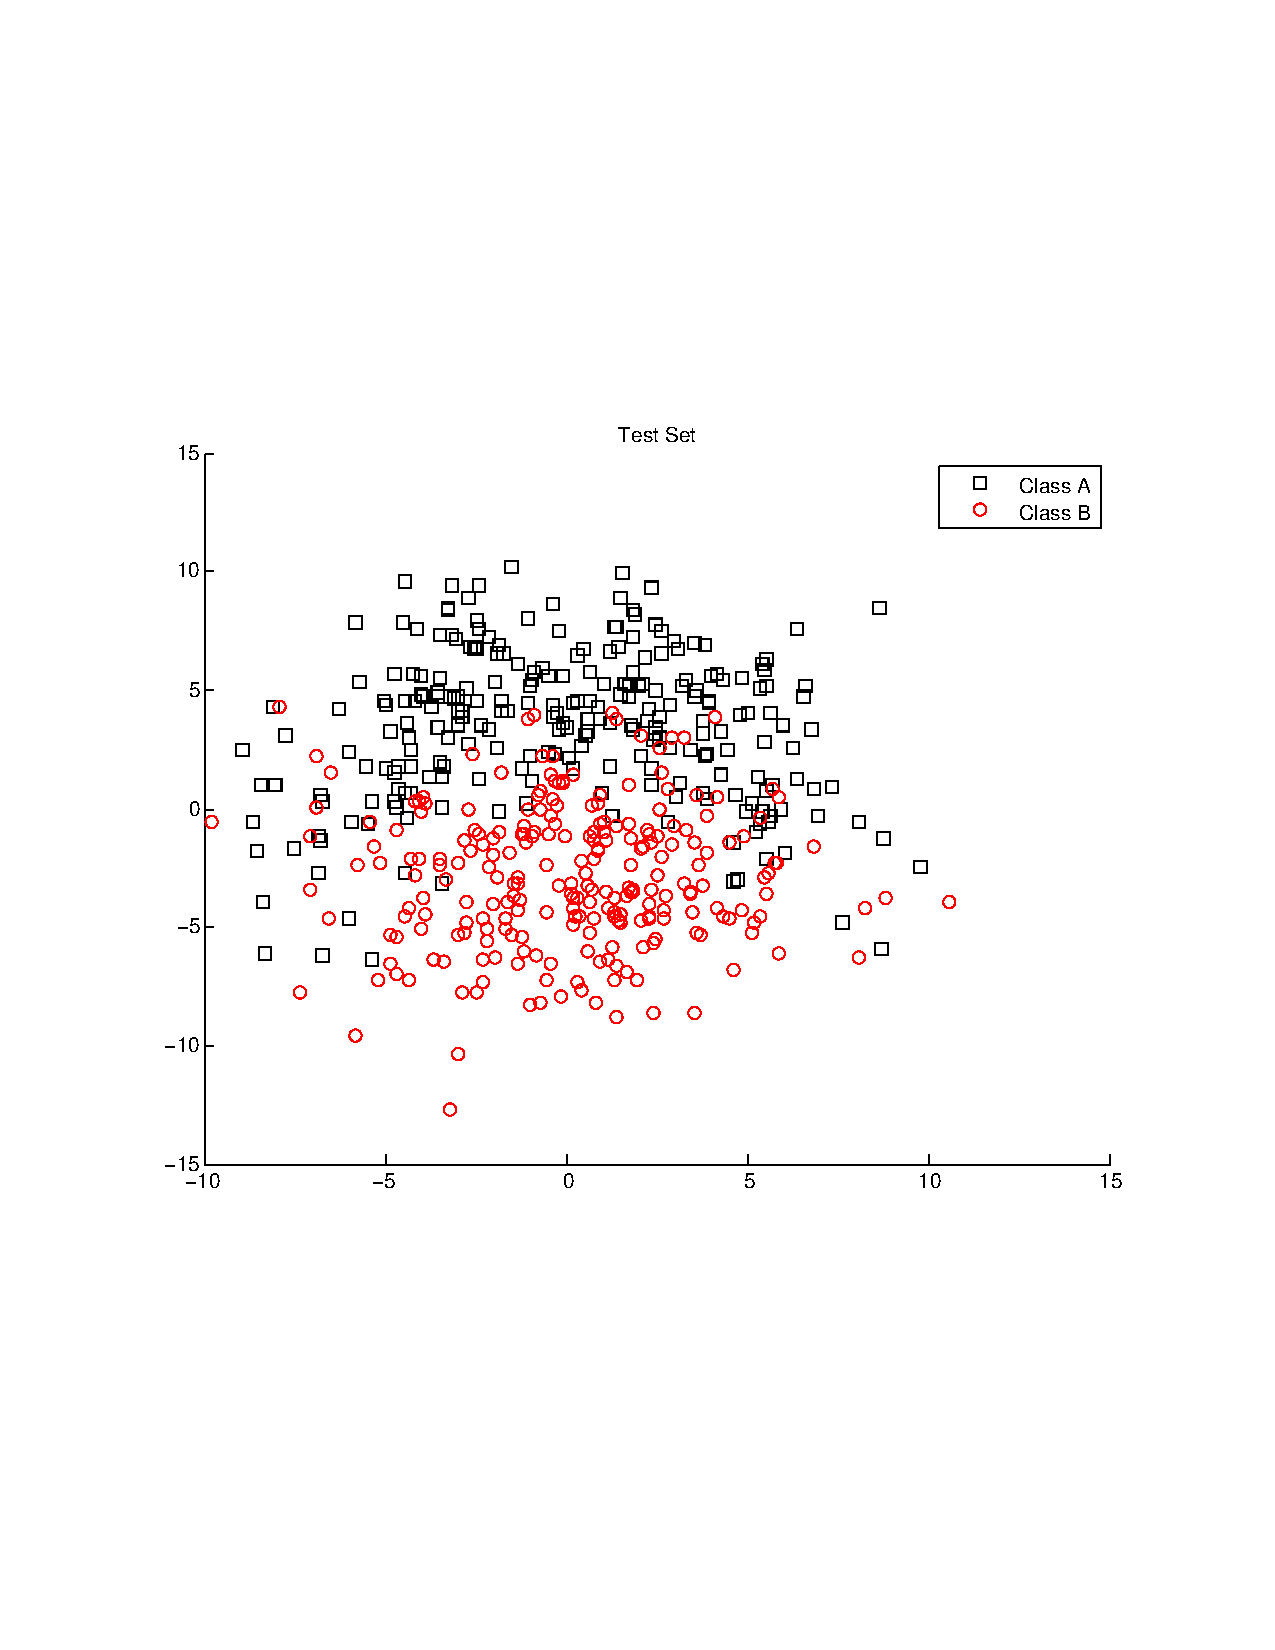
\includegraphics[trim = 0cm 7cm 0cm 7cm, clip, width=0.8\textwidth]{figures/TestSet.pdf}
  \caption{Training Set.}
  \label{fig:2}
\end{figure}


 \section*{Exercise 2}
We trained our knn classifier using the training data, evaluating its performance on the test data and computing the error rate. The error rate taking into consideration only one neighbour (k=1) was 17\%. Then we tried other values for k (k=1, 2, \ldots, 30), computing the error for each case as shown in figure.
The value of k that we would choose is k=213, because as the figure states, for k=432 the test error reaches its minimum value, on which it stabilizes in the range of k={1123,3143}, and then then increments as we increase the value of k. We were able to reach a critical conclusion regarding this experiment. As mentioned above, as the value of k increases, the test error is expected to decrease. This behavior does not refer to the whole range of k's tested values, but as k becomes significantly high the test error calculated increments aswell. We interpreted this fact as a typical case of overfitting, which is expected to occur if the value of k becomes high enough compared to the number of datapoints included in the training set.


 \section*{Exercise 3}
As described before, an overfitting problem has occurred while increasing the value of k. This might happen because either we have a model which is too complex, or the data used for training is too little. In our case, the model is relatively simple so, we should find a way to increase our training data. Here comes the solution of cross-validation. Cross-validation helps overcome overfitting while expanding the data used for training purposes. Each time we run the algorithm, a new training and test set is being used, thus giving us more accurate predictions when it comes to validation. Another algorithm we could apply in order to increase accuracy, is bootstrapping, which would at least lead us to a critical conclusion regarding the variance of the data we were given, informing us about the possible outcome of the whole simulation.
 

    \end{document}


